\documentclass{beamer}
\usetheme{default} % no fancy navigation or anything ... 
\usefonttheme{serif}   
%\usepackage{lmodern}
\usepackage{svgcolor}
\usepackage{verbatim}
\usepackage[german]{babel}
%\usepackage[latin1]{inputenc}
\usepackage{shapepar}
\usepackage{graphicx}

\title     {\LaTeX{} Mini Intro}
\author    {Tobias Oetiker}
\institute {OETIKER+PARTNER AG}
\date      {It's only the Beginning!}

\begin{document}     
\begin{frame}
  \titlepage
\end{frame}

\begin{frame}
\begin{itemize}
\item Features
\item How it works
\item \LaTeX{}-Examples
\end{itemize}
\end{frame}

\begin{frame}[fragile]{\LaTeX{} Features}
\begin{itemize}
\item Professional Standard-Layouts (WYGLRG)
\item Typesetting mathematical formul\ae
\item Logical \verb+\emph{+Mark-Up\verb+}+\\
      as opposed to optical \underline{\textbf{\textrm{Mark-Up}}}
\item Table of content, Bibliography, 
  Index, Cross references, graphics inclusion
\item Cross platform and free
\item Long-term stable language (since 1985).
\end{itemize}
\end{frame}

\begin{frame}{How \LaTeX{} Works}
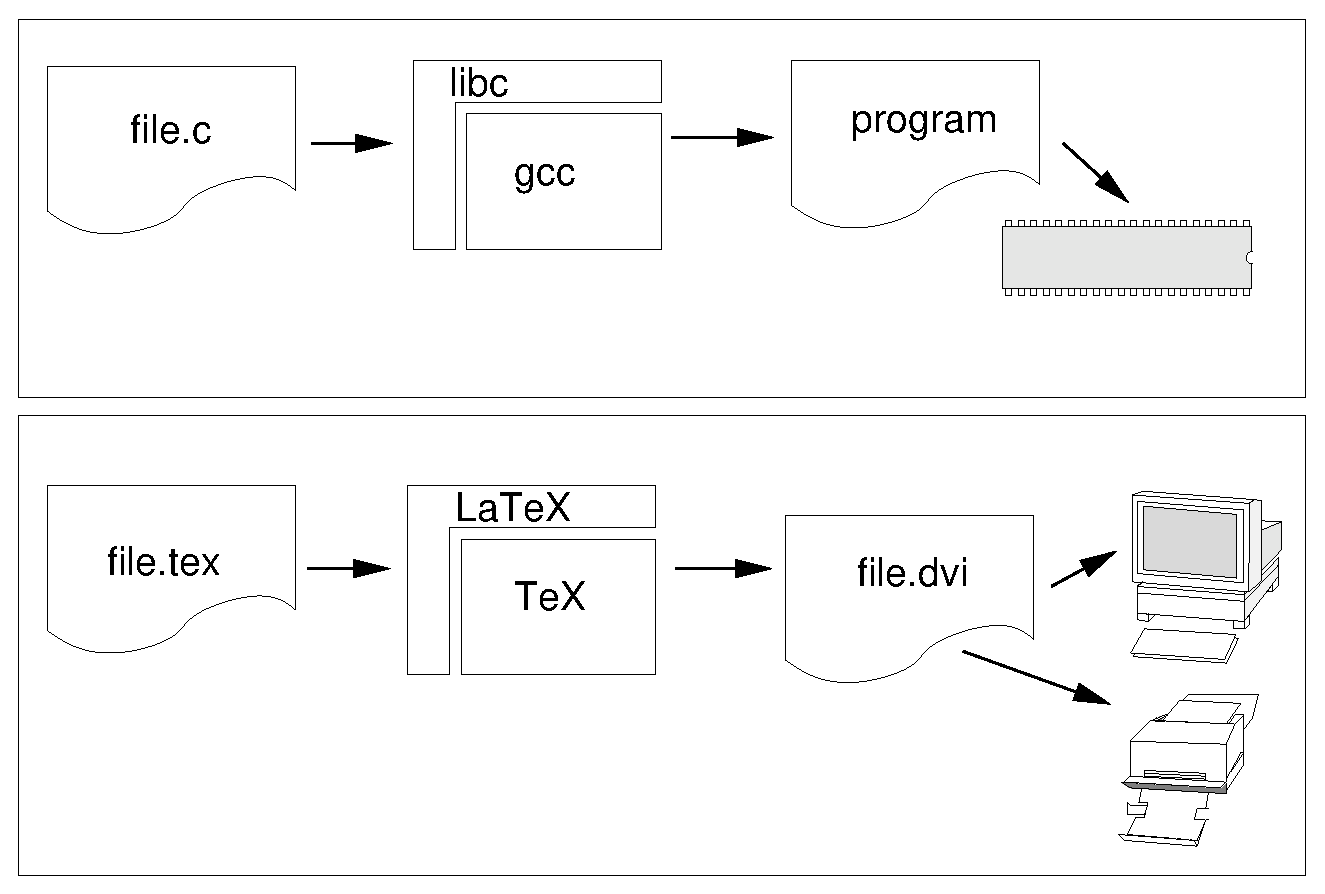
\includegraphics[width=\textwidth]{process}
\end{frame}

\begin{frame}[fragile]{Text Input}
\begin{verbatim}
\documentclass[a4paper]{article}
\usepackage[german]{babel}
\usepackage[latin1]{inputenc}
\begin{document}
\section{Lore Ipsum}
Lorem ipsum dolor sit amet, consectetur adipiscing elit.
Fusce pulvinar ante in enim rhoncus ut suscipit sapien
luctus. Sed ipsum urna, scelerisque vitae laoreet eleifend,
congue in nibh.

Nulla blandit ligula et lorem hendrerit ac tincidunt
massa scelerisque. Vestibulum vitae sem enim. Nullam
ornare consequat pellentesque. Praesent placerat,
lacus at varius auctor, magna turpis tempus tellus,
consectetur sodales metus arcu ac justo.
\end{document}
\end{verbatim}
\end{frame} 

\begin{frame}{Typeset Document}
\textbf{\large 1. Lore Ipsum}\\[1em]

Lorem ipsum dolor sit amet, consectetur adipiscing elit. Fusce pulvinar ante in enim rhoncus ut suscipit sapien luctus. Sed ipsum urna, scelerisque vitae laoreet eleifend, congue in nibh.

\hspace*{1em}Nulla blandit ligula et lorem hendrerit ac tincidunt massa scelerisque. Vestibulum vitae sem enim. Nullam ornare consequat pellentesque. Praesent placerat, lacus at varius auctor, magna turpis tempus tellus, consectetur sodales metus arcu ac justo.
\end{frame}

\begin{frame}[fragile]{Math I}

\setlength{\fboxsep}{1em}
\begin{minipage}{0.5\textwidth}
\begin{verbatim}
\frac{1}
 {\alpha_{ij} + x^2}
\end{verbatim}
\end{minipage}\hspace{1cm}%
\framebox{\parbox{0.2\textwidth}{
\begin{displaymath}
\frac{1}
{\alpha_{ij} + x^2}
\end{displaymath}}}
\end{frame}

\begin{frame}{Math II}
\begin{displaymath}
\frac{\prod _{n=1}^{\infty }(1-{x^{2 n}})}
  {\prod _{n=1}^{\infty}(1-{x^n})}
  =\sum _{k=-\infty }^{\infty }{x^{2 {k^2}+k}}
\end{displaymath}

\begin{displaymath}
\sqrt{6 + {\sqrt{6 + {\sqrt{6 + 
          {\sqrt{6 + {\sqrt{6 + 
                  {\sqrt{6 +  \cdots }}}}}}}}}}} = 3
\end{displaymath}
\end{frame}

\begin{frame}{It's only the Beginning!}

{\tiny
\heartpar{Die Gestalt des Herzens gleicht einem gut faustgro�en,
abgerundeten Kegel, dessen Spitze nach unten und etwas nach links vorne
weist. Das Herz sitzt beim Menschen in der Regel leicht nach links versetzt
hinter dem Brustbein (siehe weiter unten unter Topographie), in seltenen
F�llen nach rechts versetzt (die sogenannte Dextrokardie -
Rechtsherzigkeit), meist bei Situs inversus (spiegelverkehrter
Organanordnung).
Das gesunde Herz wiegt etwa 0,5\% des K�rpergewichts und im Durchschnitt
zwischen 300 und 350 g, wobei es bei dauerhafter Belastung eher mit der
(risikoarmen) Vergr��erung schon bestehender Herzmuskelzellen reagiert - ab
ca. 500 g, dem so genannten kritischen Herzgewicht, beginnt das Herz neben
strukturellen krankhaften Ver�nderungen bei regelm��ig auftretenden
Belastungssituationen ganz neue Herzmuskelzellen zu bilden, und es erh�ht
sich das Risiko einer absoluten Mangelversorgung der nunmehr gr��eren
Zellanzahl mit Sauerstoff, da die versorgenden Koronararterien nicht in
gleichem Ma�e mitwachsen.}}
\end{frame}

\begin{frame}{Try \LaTeX{} Online}
\url{http://www.scribtex.com}
\end{frame}

\begin{frame}{Install Texmaker Portable}
\url{http://www.xm1math.net/texmaker/texmakerwin32usb.zip}
\end{frame}

\end{document}

